\section{Data loading}\label{data-loading}

Once the database has been created, expVIP currently supports two
methods to load expression data onto the database:

\begin{enumerate}
\def\labelenumi{\arabic{enumi}.}
\itemsep1pt\parskip0pt\parsep0pt
\item
  Load the precomputed expression values into the database, or
\item
  Run Kallisto to generate the expression data. These are then loaded
  directly into the database.
\end{enumerate}

\subsection{Single big table}\label{single-big-table}

The fastest way to load the data to expVIP is to produce a table with
all the values for each expression unit (tpm, counts). The table must
contain a column \lstinline!target_id! that has the gene name, as the
first field in the fasta file used for the mapping. The rest of the
columns most contain a header with the accession of the experiment. Each
row represents a value. All the values in the table must be from the
same time.

For the case of wheat in which we have already generated the Kallisto
mapping of 418 RNA-seq studies, the expression table can be downloaded
directly from
\href{https://www.dropbox.com/sh/n15tpsqj92wfn8u/AABivEEUj4sRd9tG830WnSi4a?dl=0}{here}.
The \lstinline!txt! files are called \lstinline!final_output_counts.txt!
and \lstinline!final_output_tpm.txt! for the corresponding expression
unit.

\subsubsection{Loading from the script}\label{loading-from-the-script}

\begin{enumerate}
\def\labelenumi{\arabic{enumi}.}
\itemsep1pt\parskip0pt\parsep0pt
\item
  Double click on the \lstinline!load_values.sh!
  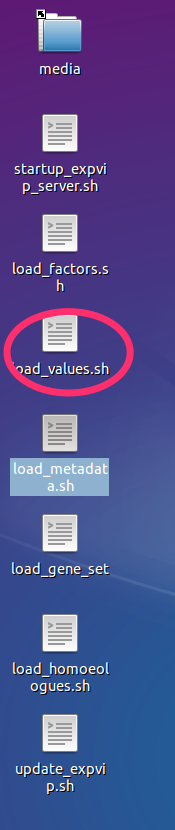
\includegraphics{images/LoadValues01.png}
\item
  Click one \lstinline!Execute in Terminal!
  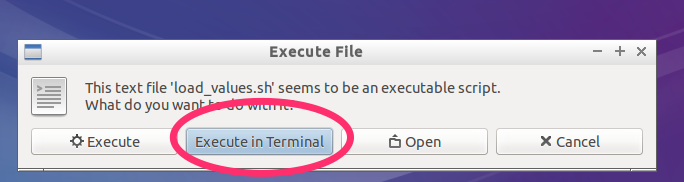
\includegraphics{images/LoadValues02.png}
\item
  Select a name for the set of alignments. expVIP can keep several runs
  of alignments in the database. The ability to select between them will
  be added in a future release.
  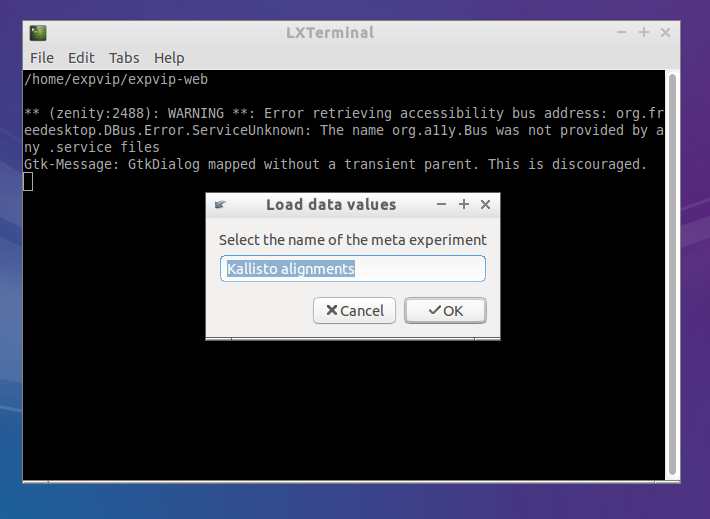
\includegraphics{images/LoadValues03.png}
\item
  The names of the gene set must be the same used when loading the
  metadata 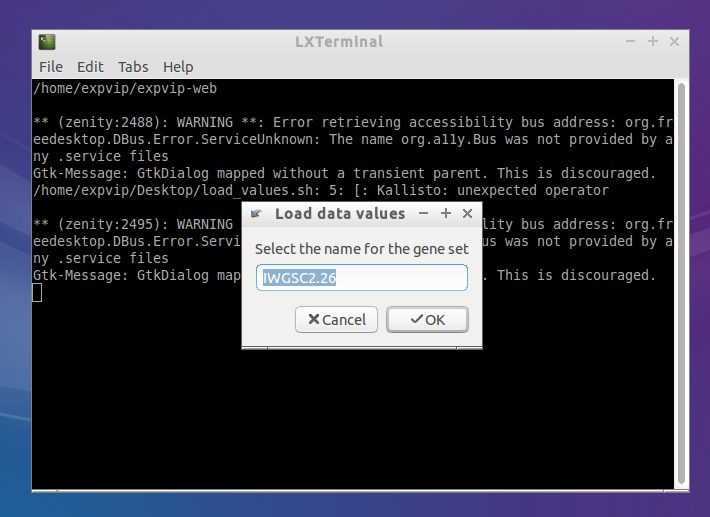
\includegraphics{images/LoadValues04.png}
\item
  Select the file with the big table. The process takes some time, so be
  patient. 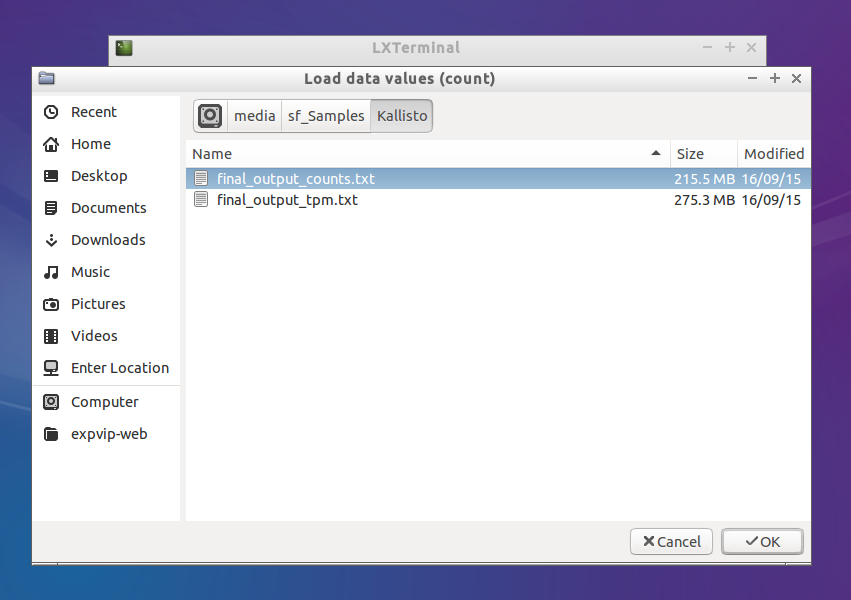
\includegraphics{images/LoadValues05.png}
\item
  An alert comes when the data finished loading.
  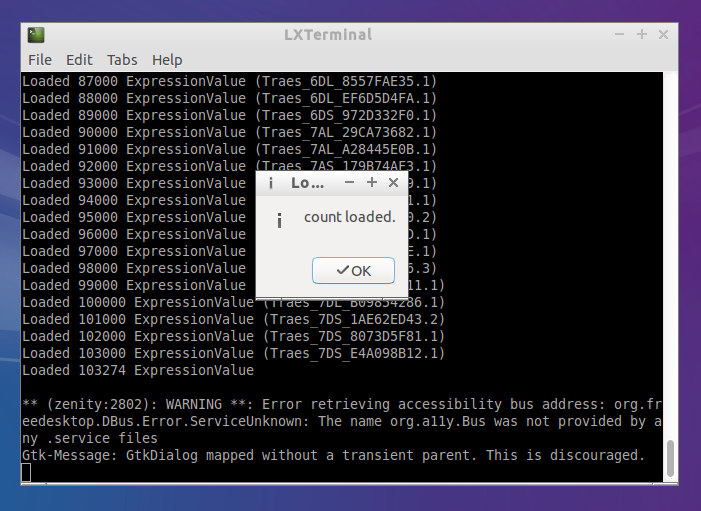
\includegraphics{images/LoadValues06.png}
\end{enumerate}

If the accession numbers are not the same as in the metadata the process
will fail.

\subsubsection{Rake Task}\label{rake-task}

In order to load the data, the task \lstinline!load_data:values! is
provided. For example, to load the tpm, the following command is used.

\begin{lstlisting}[language=sh]
rake "load_data:values[First run,IWGSC2.26,tpm,edited_final_output_tpm.txt]"
\end{lstlisting}

\subsection{Running Kallisto}\label{running-kallisto}

You can load the data directly to the database provided that you
generated the \lstinline!Kallisto! index on your reference:

\begin{lstlisting}
kallisto index --index=Triticum_aestivum.IWGSC2.26.cdna.all.fa.kallisto.k31 Triticum_aestivum.IWGSC2.26.cdna.all.fa
\end{lstlisting}

You can modify the index options as you find it suitable for your
experiment.

To run Kallisto on single sample, the following task is available:

\begin{lstlisting}
rake kallisto:runAndStorePaired[Index,folder/with/samples/ACCESSION,experiment_title,IWGSC2.26]
\end{lstlisting}

The task requires that the reads are in a folder named exactly as the
\lstinline!secondary\_study\_accession*! column in the metadata file. If
the accession doesn't exist, the task will fail.
\lstinline!experiment_title! is a name to group alignments.
